\documentclass[../main.tex]{subfiles}
\usetikzlibrary{positioning, shapes.geometric, arrows.meta}
\begin{document}

Chương 1 trình bày bối cảnh và động lực nghiên cứu của luận văn. Nội
dung chương tập trung vào bài toán phát hiện xâm nhập trên máy chủ
Linux thông qua chuỗi lời gọi hệ thống, các giới hạn của những hướng
tiếp cận hiện tại, và định hướng xây dựng Guepard Shield như một cơ
chế lai giữa mô hình học sâu và thực thi chính sách nhẹ trong nhân hệ
điều hành. Cách trình bày trong chương này nhằm làm rõ vì sao bài
toán vừa cần khả năng học từ dữ liệu, vừa cần một dạng biểu diễn đủ
đơn giản để có thể được kiểm tra tại thời điểm chạy.

\section{Đặt vấn đề}
\label{sec:dvd}

Các hệ thống máy chủ Linux hiện là nền tảng vận hành của nhiều dịch
vụ quan trọng, từ máy chủ web, cơ sở dữ liệu đến các vi dịch vụ
(microservices) trong môi trường điện toán đám mây. Vì các hệ thống
này xử lý dữ liệu và tài nguyên có giá trị, chúng thường trở thành
mục tiêu của các hành vi sau xâm nhập (post-exploitation), chẳng hạn
như thiết lập kết nối ngược (reverse shells), leo thang đặc quyền
(privilege escalation), đánh cắp dữ liệu (data exfiltration) hoặc duy
trì sự hiện diện lâu dài trong hệ thống (persistence). Dù khác nhau
về mục tiêu cụ thể, các hành vi này đều cần tương tác với nhân hệ
điều hành thông qua giao diện lời gọi hệ thống (system calls -
syscalls). Vì vậy, chuỗi syscall cung cấp một nguồn quan sát quan
trọng để mô tả hành vi của tiến trình ở ranh giới giữa không gian
người dùng (user space) và không gian hạt nhân (kernel space).

Để bảo vệ máy chủ, các hệ thống phát hiện xâm nhập trên máy chủ
(Host-based Intrusion Detection Systems - HIDS) dựa trên syscall đã
được nghiên cứu trong nhiều năm. Tuy nhiên, khi chuyển từ phát hiện
ngoại tuyến sang giám sát tại thời điểm chạy, các hệ thống này thường
gặp một đánh đổi quan trọng giữa khả năng mô hình hóa hành vi phức
tạp và chi phí thực thi. Luận văn này gọi khoảng cách đó là khoảng
cách thực thi chính sách bảo mật (enforcement gap):

\begin{enumerate}
  \item Các phương pháp phát hiện dựa trên học sâu (Deep Learning)
    như Transformer, LSTM hoặc GRU có khả năng học quan hệ ngữ cảnh
    trong chuỗi syscall và thường đạt kết quả tốt trong các thí
    nghiệm ngoại tuyến. Tuy nhiên, các mô hình này có nhiều tham số,
    cần phép toán dấu phẩy động và có độ trễ suy luận (inference
    latency) khó phù hợp với môi trường kernel. Trong bối cảnh một
    syscall cần được xử lý với chi phí rất nhỏ, việc chạy trực tiếp
    một mô hình nơ-ron trong đường đi thực thi của hệ điều hành là
    không khả thi về mặt tài nguyên và an toàn.
  \item Các hệ thống phát hiện dựa trên tập luật truyền thống (chẳng
    hạn như Falco hay Tetragon) có thể vận hành với chi phí thấp nhờ
    eBPF hoặc kernel modules. Điểm mạnh của hướng này là luật có thể
    được kiểm tra nhanh và phù hợp với cơ chế giám sát ở mức hệ
    thống. Ngược lại, phần lớn các luật được xây dựng thủ công, phụ
    thuộc vào kinh nghiệm của chuyên gia và khó bao phủ đầy đủ các
    biến thể trình tự trong dữ liệu thực tế.
\end{enumerate}

Từ các hạn chế trên, vấn đề nghiên cứu chính của luận văn là làm thế
nào để khai thác khả năng học mẫu tuần tự của mô hình học sâu, nhưng
vẫn đưa được kết quả phát hiện về một cơ chế đủ nhẹ để thực thi trong
kernel. Luận văn đề xuất \textbf{Guepard Shield}, một khung HIDS
hướng tới việc chưng cất tri thức từ mô hình Transformer thành một
biểu diễn automata hữu hạn đơn định (Deterministic Finite Automata -
DFA), sau đó triển khai bảng chuyển trạng thái này bằng eBPF\@. So với
cách chạy trực tiếp mô hình học sâu, hướng tiếp cận này đặt trọng tâm
vào việc tách giai đoạn học phức tạp ra khỏi giai đoạn thực thi thời
gian thực.

\section{Bối cảnh và các vấn đề nghiên cứu}
\label{sec:giaiphap}

Các nghiên cứu về phát hiện xâm nhập dựa trên syscall có thể được
nhìn theo nhiều hướng tiếp cận. Nhóm phương pháp ban đầu thường dựa
trên thống kê chuỗi con, tiêu biểu là STIDE (Sequence Time-Delay
Embedding) do Forrest và các cộng sự đề xuất
\cite{forrest1996sense}. STIDE lưu lại các chuỗi syscall bình thường
có độ dài cố định và đánh giá bất thường dựa trên sự xuất hiện của
những chuỗi chưa từng gặp. Cách tiếp cận này đơn giản và có chi phí
tính toán thấp, nhưng phụ thuộc mạnh vào kích thước cửa sổ $n$. Khi
hành vi của tiến trình có phụ thuộc dài hoặc nhiều nhánh thực thi hợp
lệ, mô hình n-gram dễ bỏ sót ngữ cảnh hoặc sinh cảnh báo giả.

Sự phát triển của học máy và học sâu cho phép các hệ thống HIDS học
được biểu diễn linh hoạt hơn từ dữ liệu. DeepLog
\cite{du2017deeplog}, chẳng hạn, sử dụng LSTM để dự đoán sự kiện kế
tiếp trong chuỗi log hoặc syscall. Các nghiên cứu gần đây dựa trên
Transformer và mô hình ngôn ngữ, như công trình của Fournier và các
cộng sự \cite{fournier2023language} hoặc TransCall của Al Siam và các
cộng sự \cite{alsiam2026transcall}, khai thác cơ chế tự chú ý
(Self-Attention) để mô hình hóa ngữ cảnh dài hơn. Những kết quả này
cho thấy học sâu là hướng phù hợp cho bài toán phát hiện bất thường
trình tự. Tuy nhiên, phần lớn đánh giá vẫn được thực hiện ở chế độ
ngoại tuyến, nơi mô hình có thể chạy trên CPU/GPU ở không gian người
dùng và không phải chịu các ràng buộc của kernel.

Bên cạnh các mô hình học từ dữ liệu, các công cụ giám sát hệ thống
dựa trên eBPF như Falco, Tetragon hoặc KubeArmor
\cite{her2025indepth} đã được sử dụng rộng rãi trong thực tế. Các
công cụ này phù hợp với môi trường sản xuất vì có thể quan sát sự
kiện hệ thống với chi phí thấp. Tuy nhiên, tập luật của chúng thường
được thiết kế thủ công và mang tính đặc tả. Một hướng nghiên cứu liên
quan là giải thích mô hình (XAI) và trích xuất luật (Rule Extraction)
từ mạng nơ-ron, như nghiên cứu của Abou El Houda và các cộng sự
\cite{abouelhouda2022novel} hoặc các kỹ thuật trích xuất automata từ
RNN của Weiss và các cộng sự \cite{ables2024eclectic}. Các công trình
này cung cấp gợi ý quan trọng cho việc chuyển tri thức từ mô hình
học sâu sang biểu diễn rời rạc, nhưng vẫn cần được điều chỉnh cho bài
toán syscall, kiến trúc Transformer và môi trường eBPF\@. Bảng~\ref{tab:topt}
tóm tắt các ưu điểm và hạn chế chính của các hướng
tiếp cận liên quan.

\begin{table}[htbp]
  \caption{So sánh các phương pháp phát hiện xâm nhập dựa trên syscall}
  \label{tab:topt}
  \centering
  \resizebox{\textwidth}{!}{
    \begin{tabular}{|l|p{3.5cm}|p{3.5cm}|p{2cm}|p{2cm}|}
      \hline
      \textbf{Phương pháp} & \textbf{Ưu điểm} & \textbf{Hạn chế} &
      \textbf{Khả năng học dữ liệu} & \textbf{Thực thi trong Kernel} \\ \hline
      \textbf{STIDE / N-gram} \cite{forrest1996sense} & Tốc độ nhanh,
      thuật toán đơn giản, dễ cài đặt. & Bỏ lỡ các ngữ cảnh dài hạn,
      độ chính xác thấp trên hệ thống phức tạp. & Có (Thống kê tần
      suất) & Có (Thông qua cấu trúc seccomp-BPF thô) \\ \hline
      \textbf{LSTM / DeepLog} \cite{du2017deeplog} & Nắm bắt ngữ cảnh
      động tốt hơn n-gram, độ chính xác khá tốt. & Khó xử lý song
      song khi huấn luyện, độ trễ suy luận lớn. & Có (Học sâu có giám
      sát/không giám sát) & Không phù hợp để chạy trực tiếp trong
      kernel \\ \hline
      \textbf{Transformer HIDS} \cite{fournier2023language,
      alsiam2026transcall} & Mô hình hóa tốt phụ thuộc ngữ cảnh dài,
      thường đạt kết quả phát hiện cao. & Chi phí suy luận và bộ nhớ
      lớn, khó đặt trực tiếp trên đường đi syscall. & Có (Cơ chế tự
      chú ý causal) & Không phù hợp để chạy trực tiếp trong kernel \\ \hline
      \textbf{Rules (Falco / Tetragon)} \cite{her2025indepth} & Chạy
      trực tiếp trong kernel với eBPF, độ trễ thấp. & Luật viết thủ
      công bởi chuyên gia, khó bao phủ biến thể trình tự phức tạp. &
      Không có (Tĩnh) & Có (Được thiết kế chạy trực tiếp bằng eBPF) \\ \hline
      \textbf{Guepard Shield (Đề xuất)} & Chuyển tri thức từ
      Transformer sang biểu diễn trạng thái hữu hạn để kiểm tra nhanh
      bằng eBPF. & Phụ thuộc vào chất lượng mô hình Teacher và cách
      rời rạc hóa trạng thái. & Có (Chưng cất từ Transformer Teacher)
      & Có (Thực thi bảng chuyển trạng thái
      DFA bằng eBPF Maps) \\ \hline
    \end{tabular}
  }
\end{table}

Từ bảng so sánh trên, khoảng trống chính nằm ở việc kết nối hai nhóm
khả năng: học được mẫu tuần tự từ dữ liệu và kiểm tra được mẫu đó với
chi phí thấp tại runtime. Luận văn này tập trung vào một quy trình
đầu-cuối để xấp xỉ ranh giới quyết định (decision boundary) của mô
hình Transformer bằng một biểu diễn trạng thái hữu hạn, từ đó đưa cơ
chế phát hiện về dạng có thể triển khai bằng eBPF\@.

\section{Mục tiêu nghiên cứu và Khung khái niệm}
\label{sec:muc-tieu}

Mục tiêu của luận văn là nghiên cứu và xây dựng \textbf{Guepard
Shield}, một pipeline đầu-cuối (end-to-end) cho phát hiện bất thường
dựa trên syscall. Pipeline này sử dụng mô hình Decoder-only
Transformer như mô hình Teacher để học hành vi bình thường từ dữ
liệu, sau đó chuyển biểu diễn đã học sang một DFA Student gọn hơn để
phục vụ giám sát thời gian thực. DFA không thay thế hoàn toàn năng
lực biểu diễn của Transformer, mà đóng vai trò như một xấp xỉ rời rạc
của các mẫu hành vi quan trọng, phù hợp hơn với yêu cầu thực thi bằng
eBPF trong Linux kernel.

Hệ thống được đặt trong mô hình thời gian thực theo từng luồng tiến
trình (thread-level syscall stream). Thay vì thu thập toàn bộ nhật ký
rồi phân tích ngoại tuyến, Guepard Shield duy trì trạng thái DFA cho
từng định danh luồng (Thread ID - TID) ngay trong kernel. Mỗi khi một
syscall mới xuất hiện, chương trình eBPF cập nhật trạng thái hiện tại
dựa trên bảng chuyển trạng thái đã nạp trước. Nếu chuỗi quan sát được
đưa DFA tới trạng thái không xác định hoặc trạng thái từ chối
(rejecting state), hệ thống có thể đánh dấu hành vi đó là bất thường
và chuyển sự kiện nghi vấn lên không gian người dùng để xử lý tiếp.

Quy trình nghiên cứu được chia thành 4 giai đoạn, từ chuẩn bị dữ
liệu đến thực thi trong kernel, như minh họa trong Hình~\ref{fig:pipeline}:

\begin{figure}[H]
  \centering
  \begin{tikzpicture}[
      node distance=1.5cm,
      block/.style={rectangle, draw, fill=blue!10, text width=9.5cm,
      align=center, rounded corners, minimum height=1cm, line width=0.8pt},
      line/.style={draw, -{Latex[scale=1.2]}, line width=1pt}
    ]
    % Nodes
    \node [block] (input) {\textbf{Luồng Syscall Thô (Raw Syscall Stream)}};
    \node [block, below=of input] (phase1) {\textbf{Giai đoạn 1: Tiền
      xử lý dữ liệu}\\Tokenization tên syscall (Vocabulary) \& Tạo các
    sliding windows $W$};
    \node [block, below=of phase1] (phase2) {\textbf{Giai đoạn 2:
      Transformer Teacher (Mô hình huấn luyện)}\\Decoder-only, Causal
    Self-Attention, học hành vi bình thường};
    \node [block, below=of phase2] (phase3) {\textbf{Giai đoạn 3:
      Trích xuất DFA Student}\\Phân cụm K-Means các vector ẩn $h_t$ lớp
    cuối \& Cắt tỉa thống kê (S4)};
    \node [block, below=of phase3] (phase4) {\textbf{Giai đoạn 4:
      Thực thi eBPF Kernel}\\Nạp cấu hình dfa\_config.json vào BPF Maps
    \& Giám sát thời gian thực với độ phức tạp $O(1)$};

    % Paths
    \path [line] (input) -- (phase1);
    \path [line] (phase1) -- (phase2);
    \path [line] (phase2) -- (phase3);
    \path [line] (phase3) -- (phase4);
  \end{tikzpicture}
  \caption{Sơ đồ pipeline bốn giai đoạn của hệ thống Guepard Shield}
  \label{fig:pipeline}
\end{figure}

Ngoài pipeline huấn luyện và trích xuất DFA, luận văn còn xem xét cơ
chế vận hành giữa kernel space và user space. Thành phần eBPF đảm
nhận kiểm tra nhanh trên luồng syscall, trong khi Rust Agent và
Transformer Teacher ở user space xử lý các trường hợp nghi vấn hoặc
cần đánh giá lại. Cách tổ chức này giữ đường đi runtime trong kernel
ở mức đơn giản, đồng thời vẫn cho phép hệ thống sử dụng mô hình học
sâu cho các bước phân tích nặng hơn. Sự tương tác này được mô tả
trong Hình~\ref{fig:runtime}.

\begin{figure}[H]
  \centering
  \resizebox{\textwidth}{!}{
    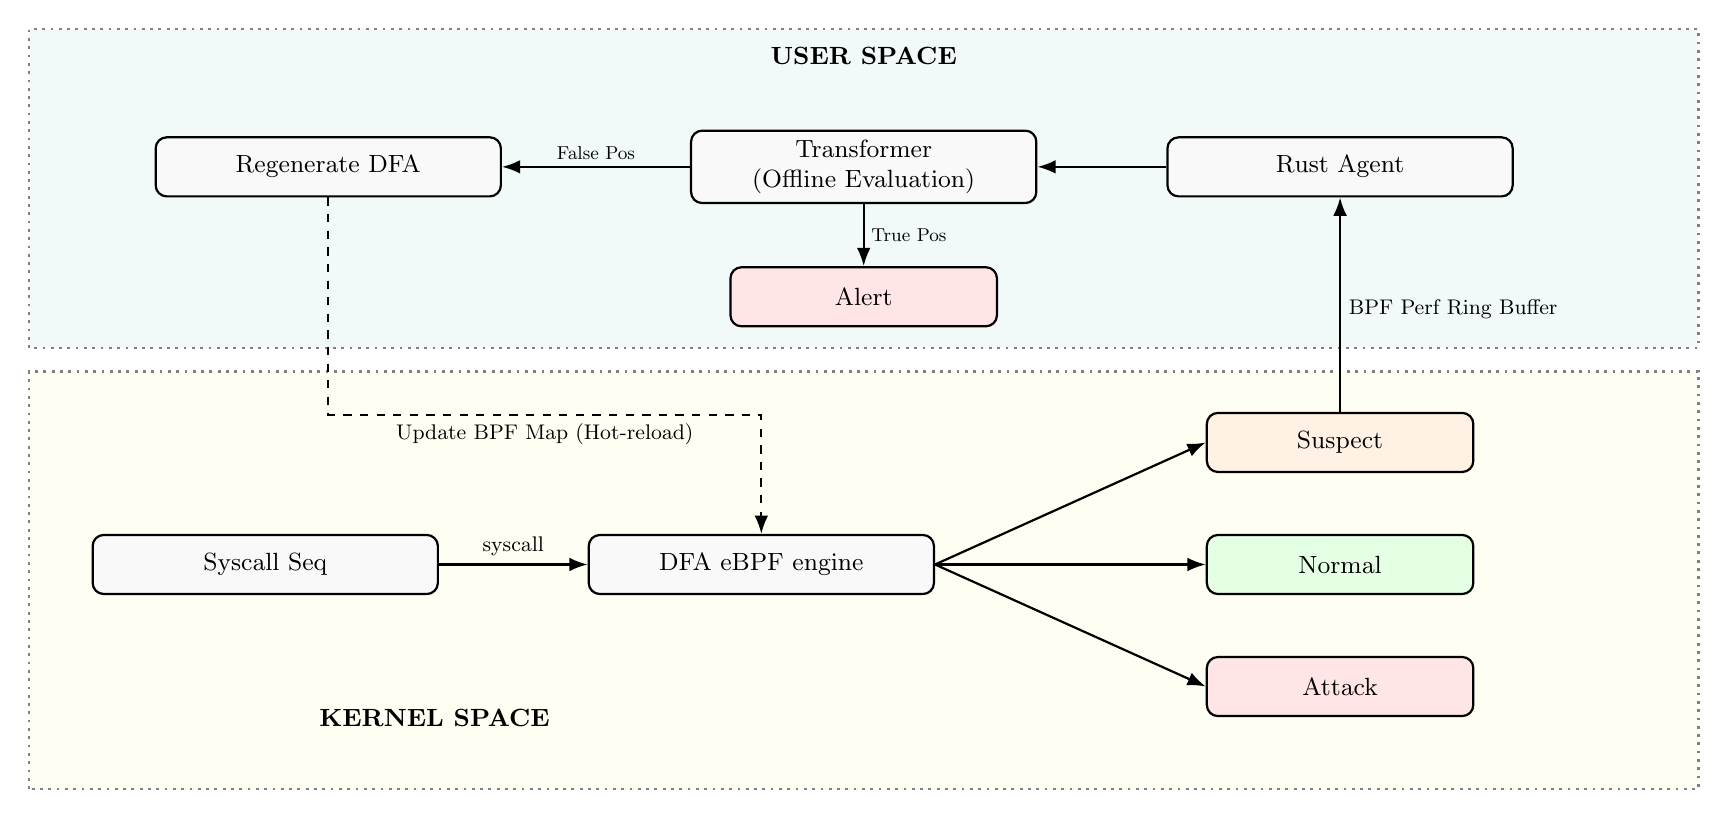
\begin{tikzpicture}[
        font=\small,
        block/.style={rectangle, draw, fill=gray!5, text
          width=4.15cm, align=center, rounded corners, minimum
        height=0.75cm, line width=0.8pt},
        action/.style={rectangle, draw, fill=red!10, text
          width=3.15cm, align=center, rounded corners, minimum
        height=0.75cm, line width=0.8pt},
        normal/.style={rectangle, draw, fill=green!10, text
          width=3.15cm, align=center, rounded corners, minimum
        height=0.75cm, line width=0.8pt},
        edge/.style={rectangle, draw, fill=orange!10, text
          width=3.15cm, align=center, rounded corners, minimum
        height=0.75cm, line width=0.8pt},
        line/.style={draw, -{Latex[scale=1.0]}, line width=0.8pt},
        dashedline/.style={draw, dashed, -{Latex[scale=1.0]}, line width=0.8pt}
      ]
      % Draw background boxes to represent Kernel and User spaces
      \draw[fill=teal!5, draw=gray, dotted, line width=1pt] (-8.0,
      -2.15) rectangle (13.2, 1.9);
      \node at (2.6, 1.56) {\textbf{USER SPACE}};

      \draw[fill=yellow!5, draw=gray, dotted, line width=1pt] (-8.0,
      -7.75) rectangle (13.2, -2.45);
      \node[fill=yellow!5, inner sep=1pt] at (-2.85, -6.85)
      {\textbf{KERNEL SPACE}};

      % User Space nodes
      \node [block] (u_agent) at (8.65, 0.15) {Rust Agent};
      \node [block] (u_teacher) at (2.6, 0.15) {Transformer
      \\(Offline Evaluation)};
      \node [block] (u_rebuild) at (-4.2, 0.15) {Regenerate DFA};
      \node [action] (u_alert) at (2.6, -1.5) {Alert};

      % Kernel Space nodes
      \node [block] (k_input) at (-5.0, -4.9) {Syscall Seq};
      \node [block] (k_dfa) at (1.3, -4.9) {DFA eBPF
      engine};

      \node [edge] (k_edge) at (8.65, -3.35) {Suspect};
      \node [normal] (k_norm) at (8.65, -4.9) {Normal};
      \node [action] (k_rej) at (8.65, -6.45) {Attack};

      % Paths in Kernel
      \path [line] (k_input) -- node[above, scale=0.85] {syscall} (k_dfa);
      \path [line] (k_dfa.east) -- (k_norm.west);
      \path [line] (k_dfa.east) -- (k_rej.west);
      \path [line] (k_dfa.east) -- (k_edge.west);

      % Path from Kernel to User Space
      \path [line] (k_edge.north)
      -- node[right, scale=0.85] {BPF Perf Ring Buffer} (8.65, -0.35)
      -- (u_agent.south);

      % Paths in User Space
      \path [line] (u_agent) -- (u_teacher);
      \path [line] (u_teacher) -- node[right, scale=0.75] {True Pos} (u_alert);
      \path [line] (u_teacher) -- node[above, scale=0.75] {False Pos}
      (u_rebuild);

      % Path from User Space back to Kernel (BPF update)
      \path [dashedline] (u_rebuild.south)
      -- (-4.2, -3.0)
      -- node[below, scale=0.85] {Update
      BPF Map (Hot-reload)} (1.3, -3.0)
      -- (k_dfa.north);

    \end{tikzpicture}
  }
  \caption{Cơ chế tương tác động và vòng lặp cập nhật giữa
  Kernel-space và User-space}
  \label{fig:runtime}
\end{figure}

Việc sử dụng DFA cho đường đi runtime có hai lý do chính:

\begin{itemize}
  \item \textbf{Độ phức tạp tính toán:} Khi mô hình Transformer thực hiện
    suy luận trên một cửa sổ trượt độ dài $W$ với số lượng lớp
    attention $L$ và chiều ẩn $d$, độ phức tạp tính toán cho mỗi bước
    dịch chuyển là $O(L \cdot W^2 \cdot d + L \cdot W \cdot d^2)$.
    Chi phí này phù hợp với huấn luyện hoặc suy luận ngoại tuyến hơn
    là với đường đi syscall trong kernel. Ngược lại, việc duyệt trạng
    thái trên DFA chỉ yêu cầu tra cứu bảng chuyển đổi và cập nhật
    trạng thái mới. Trong eBPF, thao tác này có thể được biểu diễn
    thông qua BPF map và hướng tới chi phí gần hằng số $O(1)$ cho mỗi
    sự kiện.
  \item \textbf{Tính khả thi của Verifier:} Bộ xác minh mã nguồn nhân eBPF
    (Verifier) áp đặt những giới hạn rất chặt chẽ về số lượng chỉ thị
    lệnh tối đa được thực thi trong một luồng (complexity limit),
    kích thước vùng nhớ stack chỉ 512 bytes và hạn chế các vòng
    lặp vô hạn. Một mô hình Transformer với nhiều phép toán ma trận
    và tham số học được không phù hợp với các ràng buộc này. Trái
    lại, một chương trình eBPF kiểm tra DFA có thể được viết dưới dạng
    các thao tác tra cứu và cập nhật trạng thái đơn giản, dễ đáp ứng
    hơn yêu cầu của Verifier.
\end{itemize}

\section{Các đóng góp dự kiến}
\label{sec:donggop}

Luận văn hướng tới 5 đóng góp chính sau:

\begin{enumerate}
  \item \textbf{Thiết kế pipeline HIDS đầu-cuối:} Nghiên cứu đề xuất
    một quy trình từ tiền xử lý dữ liệu syscall, huấn luyện mô hình
    Transformer causal, xây dựng DFA Student, đến triển khai bảng
    chuyển trạng thái bằng eBPF; quy trình này giúp liên kết rõ hơn
    giữa pha học từ dữ liệu và pha kiểm tra tại runtime.
  \item \textbf{Hình thức hóa phương pháp rời rạc hóa trạng thái ẩn của
    Transformer:} Luận văn xây dựng cách ánh xạ không gian embedding
    liên tục của lớp cuối Transformer (vector $h_t$) sang các trạng
    thái rời rạc của automata thông qua K-Means. Trên cơ sở đó, luận
    văn khảo sát các chiến lược xử lý tính không xác định của bước
    chuyển trạng thái, trong đó có cắt tỉa thống kê (Statistical
    Pruning, S4) đối với các bước chuyển tần suất thấp.
  \item \textbf{Phân tích khả năng chống mimicry attacks:} Luận văn
    xem xét cách các chuỗi tấn công có thể bị biến đổi bằng cách chèn
    thêm syscall bình thường (syscall padding), sau đó phân tích tác
    động của các biến đổi này lên trạng thái DFA; nội dung này giúp
    đánh giá khi nào cấu trúc whitelist của DFA có thể hỗ trợ phát
    hiện hành vi bắt chước, và khi nào cần chuyển sự kiện nghi vấn
    sang bước kiểm tra ở user space.
  \item \textbf{Đánh giá thực nghiệm trên các bộ dữ liệu syscall:}
    Luận văn đo đạc hiệu năng phát hiện của mô hình Teacher, độ trung
    thành (fidelity) của DFA Student và chi phí runtime của cơ chế
    eBPF trên các khối lượng công việc máy chủ như nginx, redis hoặc
    postgres. Các thí nghiệm này được dùng để phân tích đánh đổi giữa
    số lượng trạng thái, độ chính xác và chi phí thực thi.
  \item \textbf{Phân tích và đối sánh độ bao phủ với ma trận MITRE ATT\&CK:}
    Luận văn khảo sát khả năng ánh xạ các mẫu trạng thái bị từ chối
    trong DFA với một số kỹ thuật tấn công trong MITRE ATT\&CK, chẳng
    hạn như leo thang đặc quyền hoặc chiếm quyền điều khiển tiến
    trình. Mục tiêu của phần này là bổ sung ngữ cảnh cho cảnh báo,
    thay vì chỉ báo cáo một nhãn bất thường đơn lẻ.
\end{enumerate}

\section{Bố cục của luận văn}
\label{sec:bocuc}

Phần còn lại của luận văn được tổ chức thành 5 chương tiếp theo.

Chương 2 trình bày tổng quan tài liệu và cơ sở lý thuyết liên quan
đến bài toán giám sát an ninh mức syscall. Chương này phân tích các
phương pháp phát hiện bất thường truyền thống như STIDE, các mô hình
học sâu như DeepLog và Transformer, nền tảng automata hữu hạn đơn
định, cơ chế eBPF và các công cụ thực tế như Falco hoặc Tetragon. Từ
đó, chương làm rõ khoảng trống nghiên cứu mà luận văn hướng tới.

Chương 3 trình bày phương pháp nghiên cứu và kiến trúc của Guepard
Shield. Nội dung chính bao gồm tiền xử lý dữ liệu và token hóa tên
syscall, kiến trúc Decoder-only Transformer dùng làm Teacher, phương
pháp rời rạc hóa trạng thái ẩn bằng K-Means, cách xây dựng bảng
chuyển trạng thái DFA và thiết kế thành phần eBPF cùng Rust Agent cho
quá trình vận hành.

Chương 4 phân tích các thuộc tính lý thuyết của hệ thống. Chương này
so sánh chi phí duyệt DFA với suy luận nơ-ron trực tiếp, thảo luận
giới hạn bộ nhớ và Verifier của eBPF, phân tích khả năng xử lý
mimicry attacks và đưa ra cách đánh giá độ trung thành (fidelity) của
DFA đối với mô hình Teacher.

Chương 5 báo cáo kết quả thực nghiệm. Chương này mô tả môi trường
kiểm thử, cấu hình mô hình, các thước đo như AUROC, F1 và fidelity,
đồng thời đánh giá chi phí runtime của thành phần eBPF dưới các tải
công việc máy chủ như nginx, redis hoặc postgres.

Chương 6 tổng kết các kết quả chính của luận văn và thảo luận các
hạn chế còn lại. Chương này cũng đề xuất một số hướng phát triển tiếp
theo, bao gồm mở rộng phương pháp token hóa và cải thiện cơ chế định
tuyến các trường hợp không chắc chắn giữa kernel space và user space.

\end{document}
